\documentclass[12pt]{article}
\usepackage{amsmath,amssymb,relsize,enumitem,fancyhdr,parskip, pgfplots,multirow}
\usepackage{amsthm}
\usepackage[margin=1in]{geometry}
\usepackage{CJKutf8}
\usepackage{hyperref, comment}
\newcommand{\Z}{\mathbb{Z}}
\newcommand{\R}{\mathbb{R}}
\newcommand{\N}{\mathbb{N}}
\theoremstyle{definition}
\newtheorem{definition}{Definition}[section]
\setlength{\headheight}{28pt}
\pgfplotsset{compat=1.16}
\pagestyle{fancy}
\fancyhf{}
\setlength{\parindent}{0pt}
\fancyhead[c]{Probabilistic and Combinatorial Analysis of Rainbow Board Refresh in \begin{CJK}{UTF8}{min}パズドラ\end{CJK}}
\fancyfoot[c]{\thepage}
        
\begin{document}
\tableofcontents
\section{Introduction}
Consider the standard $6\times 5$ (6 columns, 5 rows) board in the popular mobile game \begin{CJK}{UTF8}{min}パズドラ\end{CJK}.

An $m\times n$ \textbf{board} is a array with $m$ columns and $n$ rows, where each element of the array is an \textbf{orb}. Each orb has a color (commonly chosen from a set of six colors), which is used to determine whether it is \textbf{matched}. The classical rule is that orbs are matched when 3 or more are aligned in a row or column.

\begin{definition}
    A \textbf{board refresh} refers to clearing all orbs and replacing them with randomized colors.
\end{definition}

Preliminary question: If you apply a rainbow board refresh (assuming all six standard orbs are equally probable), what is the probability of $i$ matches (including skyfalls), for $i\in\N$?
\begin{comment}
This is a deceptively hard problem as far as I can tell. I hope there is a nice closed form solution, but there probably isn't since it seems to involve partitioning.
\end{comment}

\section[2x2 board with 2-matches]{$2\times2$ board with 2-matches}
\subsection{Initial board}
Consider a simplification of the problem.
The board is now $2 \times 2$, and a match occurs when at least two orbs are adjacent (non-diagonal) to each other.

It is straightforward to enumerate all of the $6^4=1296$ possible boards, grouping them by resultant combos and board configuration.
\begin{itemize}
    \item 0 combos
    \begin{itemize}
        \item Each of the four orbs are distinct colors, so there are $\binom{6}{4}\cdot 4!=360$ boards
        \begin{center}
            \begin{tabular}{|c|c|}
            \hline
            a & b \\
            \hline
            c & d \\
            \hline
            \end{tabular}
        \end{center}
        This probability is $360/1296=5/18$.
        \item Two of the four orbs are the same color. In order to avoid matches, the two same-colored orbs are diagonal from each other. Therefore there are two possibilities.
        \begin{center}
            \begin{tabular}{|c|c|}
            \hline
            a & b \\
            \hline
            c & a \\
            \hline
            \end{tabular}
            \qquad
            \begin{tabular}{|c|c|}
            \hline
            b & a \\
            \hline
            a & c \\
            \hline
            \end{tabular}
        \end{center}
        This results in $2\cdot\binom{6}{3}\cdot 3!=240$ boards.
        This probability is $240/1296=5/27$.
        \item Two orbs are the same color and the remaining two orbs are both the same different color. To avoid matches, the same-color pairs must be diagonal from each other, and there is only a single case.
        \begin{center}
            \begin{tabular}{|c|c|}
            \hline
            a & b \\
            \hline
            b & a \\
            \hline
            \end{tabular}
        \end{center}
        This results in $\binom{6}{2}\cdot 2!=30$ boards.
        This probability is $30/1296=5/216$.
    \end{itemize}
    In total, the probability of 0 combos is $(360+240+30)/1296=35/72$.
    \item 1 combo
    \begin{itemize}
        \item With three colors, we can have the following possibilities:
        \begin{center}
            \begin{tabular}{|c|c|}
            \hline
            a & b \\
            \hline
            a & c \\
            \hline
            \end{tabular}
            \quad
            \begin{tabular}{|c|c|}
            \hline
            a & a \\
            \hline
            b & c \\
            \hline
            \end{tabular}
            \quad
            \begin{tabular}{|c|c|}
            \hline
            b & c \\
            \hline
            a & a \\
            \hline
            \end{tabular}
            \quad
            \begin{tabular}{|c|c|}
            \hline
            b & a \\
            \hline
            c & a \\
            \hline
            \end{tabular}
        \end{center}
        This results in $4\cdot \binom{6}{3}\cdot 3!=480$ boards.
        \item WIth two colors, we have the following possibilities:
        \begin{center}
            \begin{tabular}{|c|c|}
            \hline
            a & a \\
            \hline
            a & b \\
            \hline
            \end{tabular}
            \quad
            \begin{tabular}{|c|c|}
            \hline
            a & a \\
            \hline
            b & a \\
            \hline
            \end{tabular}
            \quad
            \begin{tabular}{|c|c|}
            \hline
            b & a \\
            \hline
            a & a \\
            \hline
            \end{tabular}
            \quad
            \begin{tabular}{|c|c|}
            \hline
            a & b \\
            \hline
            a & a \\
            \hline
            \end{tabular}
        \end{center}
        This results in $4\cdot \binom{6}{2}\cdot 2!=120$ boards.
        \item 
        If all four orbs are the same color, there is only one configuration and $6$ possible boards.
    \end{itemize}
    In total, the probability of 1 combo is $(480+120+6)/1296=101/216$.
    \item 2 combo
    \begin{itemize}
        \item Two adjacent orbs are the same color, and the other two adjacent orbs are another same color.
        \begin{center}
            \begin{tabular}{|c|c|}
            \hline
            a & b \\
            \hline
            a & b \\
            \hline
            \end{tabular}
            \qquad
            \begin{tabular}{|c|c|}
            \hline
            a & a \\
            \hline
            b & b \\
            \hline
            \end{tabular}
        \end{center}
        This results in $2\cdot\binom{6}{2}\cdot 2!=60$ boards.
    \end{itemize}
    The probability of 2 combos is $60/1296=5/108$.
\end{itemize}
\begin{center}
\begin{tikzpicture}
\begin{axis}[
    title=Initial Distribution,
	ylabel=Probability,
	ymax=1,
	enlargelimits=0.15,
	ybar,
	xtick=data,
	xlabel=Combos
]
\addplot coordinates {(0, 35/72) (1, 101/216) (2, 5/108)};
\end{axis}
\end{tikzpicture}
\end{center}
This distribution is consistent with Monte Carlo simulations.
\subsection{Skyfalls enabled}
Now we can consider the board configurations as states of a discrete-time stochastic process. The first thing we should figure out is if this process is Markovian. (Of course it is, since all predictive information about future combos is obtained by the current state of the board.) Another thing to consider is the fact that the number of combos is unbounded when skyfalls are enabled, but the expected number of combos is finite.

The best way to assign states is probably the distinct board configurations as listed above.

\begin{itemize}
    \item 0 combo
    \begin{itemize}
        \item Clearly the boards with 0 matches/combos are absorbing states as they do not give rise to any skyfalls, let alone skyfall combos. Any prior board information does not impact the future states since there cannot be any skyfalls.
    \end{itemize}
    \item 1 combo
    \begin{itemize}
        \item The three color case leads to three distinct possible remainder boards.
        \begin{center}
            \begin{tabular}{|c|c|}
            \hline
             &  \\
            \hline
            a & b \\
            \hline
            \end{tabular}
            \qquad
            \begin{tabular}{|c|c|}
            \hline
            a & \phantom{a} \\
            \hline
            b & \phantom{a} \\
            \hline
            \end{tabular}
            \qquad
            \begin{tabular}{|c|c|}
            \hline
            \phantom{a} & a \\
            \hline
            \phantom{a} & b \\
            \hline
            \end{tabular}
        \end{center}
        The first board occurs with conditional probability $1/2$, while the other two each occur with probability $1/4$.
        
        In the first subcase, the bottom two orbs are different. This eliminates the possibility of half of the overall 60 possible 2-combo boards, as well as $480/4+120/2+6=186$ of the possible 1-combo boards, leaving 420 remaining 1-combo boards. Note that the total possible boards where the bottom two orbs are different is $5\cdot 6^3=1080$. Therefore, the probabilities for the subsequent number of combos in the first subcase are as follows:
        \begin{center}
            \begin{tabular}{|c|c|}
            \hline
            Combos & Probability \\
            \hline
            0 & 630/1080 \\
            \hline
            1 & 420/1080 \\
            \hline
            2 & 30/1080 \\
            \hline
            \end{tabular}
        \end{center}
        The other two subcases are identical since they are simply rotations of the first subcase.
        
        Of the remaining 420 possible 1-combo boards, the 60 boards with two colors result in an identical distribution to a full board refresh, while the other 360 have two adjacent orbs fixed.
        
        Note that the conditional probability of this three color case is $480/606=80/101$.

        \item 
        The two color case with a single combo results in a single remainder orb at the lower left or lower right, each with equal probability. The color of the remainder orb is known, but no other information about the board configuration is known. Therefore all of the initial boards, restricted to those with the appropriate color assignments are possible. That is, we think about all the possible boards and divide by six to exclude those with the inconsistent remainder orb. This implies that the transition probabilities are identical to a full board refresh.
        \item The single color case is equivalent to a complete board refresh. Therefore all of the initial boards are once again equally likely. Prior information about the board is irrelevant.
    \end{itemize}
    \item 2 combo
    \begin{itemize}
        \item All of the orbs are cleared, so the initial boards are all equally likely. Prior information about the board is irrelevant.
    \end{itemize}
\end{itemize}
With this information, let $x$ be the expected number of combos, including those contributed by skyfalls. Then we have
\begin{multline*}
    x = (35/72)0 + (606/1296)[1+(480/606)((630/1080)0 \\
    +(420/1080)(1+(1/7)x+(6/7)y)+(30/1080)(2+x))+(126/606)x] + (5/108)(2+x)
\end{multline*}

where $y$ is the expected number of combos when two adjacent orbs are fixed. Moreover,
\begin{comment}
\begin{multline*}
    y = (630/1080)(0)+(420/1080)[1+(80/101)((1/7)x+(6/7)y)+(21/101)x] \\
    +(30/1080)(2+x)
\end{multline*}
\begin{multline*}
    y = (630/1080)(0)+(420/1080)[1+(60/420)x+(360/420)y] \\
    +(30/1080)(2+x)
\end{multline*}
\end{comment}
\begin{align*}
    y=(630/1080)0
    +(420/1080)(1+(1/7)x+(6/7)y)
    +(30/1080)(2+x)
\end{align*}

Solving this system of equations yields $x = 523/525$.

Simulation with ten million trials yields an average of 0.9968951 combos.

\subsection{Poison, mortal poison, jammer, bomb orbs enabled}
What if we want to consider more than just the six standard orb colors? If we generalize to $c$ colors, the number of boards increases to $c^4$ boards. However, the same analysis of board configurations as before works, replacing all instances of 6 with $c$, as long as $c\geq 2\times 2$. If $c<4$, then the possible board configurations changes, along with their associated probabilities.

For $c\geq 4$, we find the distribution for the initial board. Applying the same analysis as above results in the following:
\begin{center}
    \renewcommand{\arraystretch}{2}
    \begin{tabular}{|c|c|}
        \hline
        Number of Combos & Probability \\
        \hline\hline
        0 & $\left[\binom{c}{4}\cdot 4! + 2 \cdot \binom{c}{3}\cdot 3! + \binom{c}{2} \cdot 2!\right]/c^4$\\
        \hline
        1 & $\left[4\cdot \binom{c}{3}\cdot 3!+4\cdot\binom{c}{2}\cdot 2! + c\right]/c^4$ \\
        \hline
        2 & $\left[2\cdot\binom{c}{2}\cdot 2!\right]/c^4$\\
        \hline
    \end{tabular}
    \renewcommand{\arraystretch}{2}
\end{center}
For example, the distribution for various values of $c$ is given below (probabilities rounded to 3 decimal places):
\begin{center}
    \begin{tabular}{|c|c|c|c|}
        \hline
        \multirow{2}{9em}{Number of Combos} & \multicolumn{3}{|c|}{Probability} \\
        \cline{2-4}
         & $c=4$ & $c=7$ & $c=9$\\
        \hline\hline
        0 & $0.328$ & $0.542$ & $0.626$\\
        \hline
        1 & $0.578$ & $0.423$ & $0.353$\\
        \hline
        2 & $0.094$ & $0.035$ & $0.022$\\
        \hline
    \end{tabular}
    \quad
\end{center}
As a bonus, this enumerative method provides a nice identity:
\begin{align*}
    c^4 &= \binom{c}{4}\cdot 4! + 2 \cdot \binom{c}{3}\cdot 3! + \binom{c}{2} \cdot 2! + 4\cdot \binom{c}{3}\cdot 3!+4\cdot\binom{c}{2}\cdot 2! + c + 2\cdot\binom{c}{2}\cdot 2!\\
    &= c(c-1)(c-2)(c-3)+6c(c-1)(c-2)+7c(c-1)+c
\end{align*}

Keep in mind this also assumes the $c$ different orb colors are assumed to be equally probable. Otherwise, the problem gets even more complicated.

\section[3x3 board with 3-matches]{$3\times 3$ board with 3-matches}
Before returning to the classical problem, we consider a $3\times 3$ board to avoid dealing with cascades.

Let $c$ be the number of colors. Note that there are $c^9$ distinct boards.

We repeat the same enumerative process as before.
\begin{itemize}
    \item 0 combos
    \item 1 combo
    \item 2 combos
    \begin{itemize}
        \item The two color case
    \end{itemize}
    \item 3 combos
    \begin{itemize}
        \item With two colors, there are two board configurations, similar to the $2\times 2$ case.
        \begin{center}
            \begin{tabular}{|c|c|c|}
                \hline
                a & a & a \\
                \hline
                b & b & b \\
                \hline
                a & a & a \\
                \hline
            \end{tabular}
            \qquad\qquad
            \begin{tabular}{|c|c|c|}
                \hline
                a & b & a \\
                \hline
                a & b & a \\
                \hline
                a & b & a \\
                \hline
            \end{tabular}
        \end{center}
        This results in $2\cdot \binom{c}{2}\cdot 2!$ boards. For $c=6$, this amounts to 60 boards.
        \item With three colors, there are two similar board configurations, similar to the $2\times 2$ case.
        \begin{center}
            \begin{tabular}{|c|c|c|}
                \hline
                a & a & a \\
                \hline
                b & b & b \\
                \hline
                c & c & c \\
                \hline
            \end{tabular}
            \qquad\qquad
            \begin{tabular}{|c|c|c|}
                \hline
                a & b & c \\
                \hline
                a & b & c \\
                \hline
                a & b & c \\
                \hline
            \end{tabular}
        \end{center}
        This results in $2\cdot \binom{c}{3}\cdot 3!$ boards. For $c=6$, this amounts to 240 boards.
    \end{itemize}
    In total, there are $2\cdot \binom{c}{2}\cdot 2!+2\cdot \binom{c}{3}\cdot 3!$. With six available colors, the probability of 3 combos is $300/6^9\approx 0.0000298$.
\end{itemize}
With $c=6$ colors, the approximate distribution for initial board is as follows.
The approximate distribution from Monte Carlo simulation is as follows:
\begin{center}
\begin{tabular}{|c|c|}
    \hline
    Combos & Approximate Probability \\
    \hline\hline
    0 combos & 0.844341 \\
    \hline
    1 combo & 0.151848 \\
    \hline
    2 combos & 0.003783 \\
    \hline
    3 combos & 0.000028 \\
    \hline
\end{tabular}
\end{center}
\section[6x5 board with 3-matches]{$6\times 5$ board with 3-matches}
We return to the classical problem on a $6\times 5$ board, allowing 3-matches.


\subsection{Classifying boards based on number of colors}

Here we count all the boards with exactly $i$ number of colors for $i=1,\dots,6$ and compute the probabilities of occurrence after a random board refresh. Note that the total number of boards is $6^{5\times 6}=6^{30}$.

If a board is monocolor, there are $\binom{6}{1}$ boards, since we choose one color from the possible six. Thus the probability of occurrence is $\binom{6}{1}/6^{30}$.

How many distinct bicolor boards are there? Since we can choose two out of six colors and one of the two colors for each orb, there are $\binom{6}{2}\cdot 2^{30}$ boards with at most two colors. This includes all of the monocolor boards, so number of strictly bicolor boards is $\binom{6}{2}\cdot 2^{30}-\binom{6}{1}$.

In a similar fashion, the number of boards with exactly $i$ colors is $\binom{6}{i}\cdot i^{30}-\binom{6}{i-1}\cdot (i-1)^{30}$. The probability of having a board with $i$ colors is $\left[\binom{6}{i}\cdot i^{30}-\binom{6}{i-1}\cdot (i-1)^{30}\right]/6^{30}$.

\begin{center}
\renewcommand{\arraystretch}{2}
    \begin{tabular}{|c|c|c|}
        \hline
        Number of Colors & Number of Boards & Approximate Probability \\
        \hline\hline
        $1$ & $\binom{6}{1}$ & $%\binom{6}{1}/6^{30}\approx 
        2.71\times 10^{-23}$ \\
        \hline
        $2$ & $\binom{6}{2}\cdot 2^{30}-\binom{6}{1}$ & $%\left[\binom{6}{2}\cdot 2^{30}-\binom{6}{1}\right]/6^{30}\approx
        7.29\times 10^{-14}$ \\
        \hline
        $3$ & $\binom{6}{3}\cdot 3^{30}-\binom{6}{2}\cdot 2^{30}$ & $%\left[\binom{6}{3}\cdot 3^{30}-\binom{6}{2}\cdot 2^{30}\right]/6^{30}\approx 
        1.86\times 10^{-8}$ \\
        \hline
        $4$ & $\binom{6}{4}\cdot 4^{30}-\binom{6}{3}\cdot 3^{30}$ & $%\left[\binom{6}{4}\cdot 4^{30}-\binom{6}{3}\cdot 3^{30}\right]/6^{30}\approx 
        7.82\times 10^{-5}$ \\
        \hline
        $5$ & $\binom{6}{5}\cdot 5^{30}-\binom{6}{4}\cdot 4^{30}$ & $%\left[\binom{6}{5}\cdot 5^{30}-\binom{6}{4}\cdot 4^{30}\right]/6^{30}\approx 
        2.52\times 10^{-2}$ \\
        \hline
        $6$ & $\binom{6}{6}\cdot 6^{30}-\binom{6}{5}\cdot 5^{30}$ & $%\left[\binom{6}{6}\cdot 6^{30}-\binom{6}{5}\cdot 5^{30}\right]/6^{30}\approx 
        0.975$ \\
        \hline
    \end{tabular}
\renewcommand{\arraystretch}{2}
\end{center}
These exact probabilities indicate that it is extremely likely to end up with a board containing five or six colors, while monocolor, bicolor, tricolor, and quadcolor boards almost never occur. 

\begin{definition}
    A board is called \textbf{rainbow matchable} if it contains at least 3 orbs of each color.
\end{definition}

A few natural questions arise:
\begin{enumerate}
    \item Unconditionally (that is, a board with or without preexisting matches), what is the probability that the board is rainbow matchable?
    \item Given a 0 combo board, what is the probability that the board is rainbow matchable.?
\end{enumerate}
At first glance, the answer to these two problems might seem like they should be identical. However, maybe it is possible that 0 combo boards increase (or decrease) the likelihood because some configurations are favored. For example when considering 0 combo boards, monocolor boards are excluded entirely, and the majority of bicolor and tricolor boards are excluded as well.
\subsection{Classifying monocolor boards}
There are only six of them, each resulting in another board refresh. This subsection is only included for completeness.
\subsection{Classifying bicolor boards}
We know there are $\binom{6}{2}\cdot 2^{30}-\binom{6}{1}$ bicolor boards from earlier.

If we fix the two colors, there are only $2^{30}-2$ distinct board configurations. ???
% Am I somehow miscounting? Because there is symmetry between two colors
\subsection{Average number of natural explicit combos}
Natural means all distinct boards are equally likely. Explicit means no implicit combos due to skyfalls or cascades.

After doing Monte Carlo simulation with 10 million trials, we find the average number of combos is approximately 0.8557792.

The approximate distribution is as follows:
\begin{center}
\begin{tabular}{|c|c|}
    \hline
    Combos & Approximate Probability \\
    \hline\hline
    0 combos & 0.3793952 \\
    \hline
    1 combo & 0.422572 \\
    \hline
    2 combos & 0.1651948 \\
    \hline
    3 combos & 0.0299233 \\
    \hline
    4 combos & 0.0027802 \\
    \hline
    5 combos & 0.000132 \\
    \hline
    6 combos & 0.0000025 \\
    \hline
    7 combos & 0 \\
    \hline
    8 combos & 0 \\
    \hline
    9 combos & 0 \\
    \hline
    10 combos & 0 \\
    \hline
\end{tabular}
\end{center}
\begin{center}
\begin{tikzpicture}
\begin{axis}[
    title=Simulated Initial Distribution,
	ylabel=Probability,
	ymax=1,
	enlargelimits=0.15,
	ybar,
	xtick=data,
	xlabel=Combos
]
\addplot coordinates {(0, 0.3793952) (1, 0.422572) (2, 0.1651948) (3, 0.0299233) (4, 0.0027802) (5, 0.000132) (6, 0.0000025) (7, 0) (8, 0) (9, 0) (10, 0)};
\end{axis}
\end{tikzpicture}
\end{center}
The exact values? Find out on the next episode of \textit{Cases: The Tragedy}.

\subsection{Skyfalls enabled}
After running simulations, the average number of combos with skyfalls and cascades is somewhere around 1.14.

The approximate distribute is as follows:

\begin{center}
\begin{tikzpicture}
\begin{axis}[
    title=Simulated Distribution (Skyfalls Enabled),
	ylabel=Probability,
	ymax=1,
	enlargelimits=0.15,
	ybar,
	xtick=data,
	xlabel=Combos
]
\addplot coordinates {(0, 0.38173) (1, 0.31114) (2, 0.17394) (3, 0.08024) (4, 0.03314) (5, 0.01254) (6, 0.00469) (7, 0.00146) (8, 0.00078) (9, 0.00023) (10, 0.0001)};
\end{axis}
\end{tikzpicture}
\end{center}

\section[mxn board with k-matches]{$m\times n$ board with $k$-matches}
I don't know if this is even possible to study further than running a few Monte Carlo simulations. Combinatorics is hard.
\section{Appendix}
\subsection{Algorithm Used to Count Matches}
The algorithm can be found at this \href{https://github.com/jli0108/jli0108.github.io/blob/master/pazudora-simulation/index.html}{link}.

The idea is to look at each orb that has not already been checked (this information is stored in \verb|checkedMatches|). Using the function \verb|checkMatches|, the algorithm checks all possible ways in which the reference orb can be part of a 3-match. The matches only contribute to combo count if none of the orbs that are part of the match have been previously matched (this information is stored in \verb|matched|). In order to avoid overcounting combos in edge case configurations, the function \verb|checkMatches| must label all orbs that are connected to the 3-match before moving on to another match. For this reason, the function checkes for any adjacent orbs with the same color as the reference orb and recursively calls itself (if the \verb|checkedMatches| field is false).
\end{document}